\section{Demonstration}

  In this chapter, the following procedure will be demonstrated as the result of this research project:

  \begin{itemize}
   \item Retrieve a list of existing validation rules
   \item Creating a runtime secret (API key) to be used in one of the validation rule 
   \item Create a new validation rule
   \item Retrieve a list of validation processes
   \item Schedule a new validation process
   \item Email a specified email address if the fraud score of the validation exceeds \verb;0.5;
  \end{itemize}

  For demonstration purposes, an AMQP consumer is implemented to email a specified email address if the fraud exceeds a certain number\footnote{The AMQP consumer for the demonstration purpose is available as an attachment to this thesis}. Furthermore, an external address verification API\footnote{The external address validation used for the demonstration is Lob address verification. Homepage: \url{https://www.lob.com/address-verification}.} will be used as the external service for this demonstration. Therefore, an API key for the corresponding API needs to be created and added to the runtime secret of the validation engine. 

  After running the application using the command \verb;docker-compose up;, the UI is accessible on \verb;http://localhost:3000; and the FDS is accessible on \verb;http://localhost:8000;. The URL \verb;http://localhost:3000/#/rules; can be visited to display the list of available validation rules in the database. A new runtime secret can be created from the rules list page by clicking the \textsc{Secrets} button and then \textsc{Create a new secret} button afterward. 

  \begin{figure}[!ht]
   \centering
   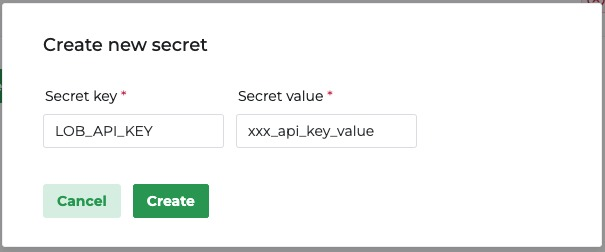
\includegraphics[width=0.6\textwidth]{images/create_secret.jpeg}
   \caption{Screenshot of a runtime secret creation}
  \end{figure}

  The lob API uses the \emph{Basic Auth} authentication scheme, which requires a client to send the \verb;Authorization; header that contains the \verb;Basic ; prefix, followed by the base64 encoded value of the Lob API key. As the runtime secret is created, it is now accessible to the validation rule using the \verb;$.secrets.LOB_API_KEY; JSONPath expression. A new validation rule is created by clicking on the \textsc{Add new rule} button. A rule management form is displayed, and the user can enter the values to each attribute of the validation rule. For the demonstration, the following validation rule is created: 

  \begin{itemize}
   \item Name: "Address Validation"
   \item Endpoint: \verb;https://api.lob.com/v1/intl_verifications;
   \item HTTP method: \verb;POST;
   \item Fail score: 0.5
   \item Request body: 
     \begin{itemize}
       \item \verb;recipient: "FDS";
       \item \verb;primary_line: $.customer.address.street;
       \item \verb;city: $.customer.address.city;
       \item \verb;state: $.customer.address.state;
       \item \verb;country: $.customer.address.country;
     \end{itemize}
   \item Request header: \verb;Authorization: Basic $.secrets.LOB_API_KEY;
   \item Conditions:
     \begin{itemize}
      \item Evaluate whether the status code equals to 200
      \item Evaluate whether the response body returns a \verb;valid_address; attribute and whether it equals to \verb;true;
     \end{itemize}
  \end{itemize}
  
  By visiting the URL \verb;http://localhost:3000/#/validations;, the list of ongoing and completed validation processes, saved in the data store of FDS will be displayed. A new validation process can be created by clicking on the \textsc{Create new validation} button and filling in the validation form with a sample customer data, on which a validation process should be executed. As mentioned before, several sample customers with different attributes are created to provide an even easier testing process. For the demonstration purpose, the user with the label \verb;Berlin-based customer (invalid address); will be chosen, as it will trigger a failed rule evaluation of the \verb;Address Validation; validation rule. 

  \begin{figure}[!ht]
   \centering
   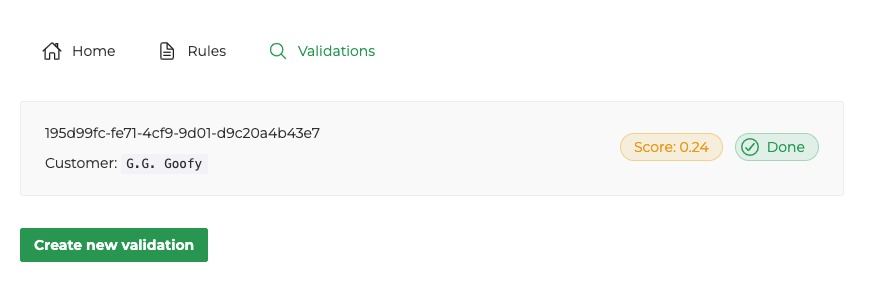
\includegraphics[width=\textwidth]{images/ss_validation_list.jpeg}
   \caption{Screenshot of the validation list page}
  \end{figure}

  After filling the validation form with a sample customer data, a validation process will be scheduled by clicking on the \textsc{Validate customer} button. As a validation process is scheduled, the user will be redirected to a validation process page, on which the progress of the validation process will be displayed in real-time. 

  Upon the completion of the validation process, validation result should return a \verb;0.5; fraud score, as the sample customer's address is invalid. As mentioned earlier, a certain action should be done by the AMQP consumer, when there's a validation process that resulted in a fraud score of \verb;0.5;. An email should be sent to the email address, specified when running the AMQP consumer. 
  
  \begin{figure}[!ht]
   \centering
   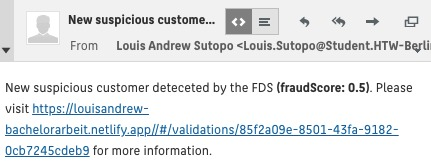
\includegraphics[width=0.6\textwidth]{images/ss_email.jpeg}
   \caption{Screenshot of an email sent by AMQP consumer when a validation process completed with a fraud score exceeding 0.5}
  \end{figure}